\documentclass[14pt,a4paper]{article}

% ── Packages ──────────────────────────────────────────────
\usepackage[utf8]{inputenc}
\usepackage[T1]{fontenc}
\usepackage[french]{babel}
\usepackage{geometry}
\usepackage{graphicx}
\usepackage{float}
\usepackage{xcolor}
\usepackage{listings}
\usepackage{fancyhdr}
\usepackage{titlesec}
\usepackage{hyperref}
\usepackage{booktabs}
\usepackage{amsmath}
\usepackage{enumitem}
\usepackage{tcolorbox}
\usepackage{mdframed}
\usepackage{caption}
\usepackage{subcaption}

\setlength{\parindent}{1.5em}
\setlength{\parskip}{0pt}

% ── Page geometry ─────────────────────────────────────────
\geometry{margin=2.5cm, top=3cm, bottom=3cm}

% ── Colors ────────────────────────────────────────────────
\definecolor{darkblue}{HTML}{1a237e}
\definecolor{medblue}{HTML}{1565c0}
\definecolor{askbg}{HTML}{e3f2fd}
\definecolor{codegreen}{HTML}{2e7d32}
\definecolor{codegray}{HTML}{546e7a}
\definecolor{codebg}{HTML}{f5f5f5}
\definecolor{answerbg}{HTML}{e8f5e9}
\definecolor{answerframe}{HTML}{2e7d32}
\definecolor{notebg}{HTML}{ede7f6}
\definecolor{noteframe}{HTML}{4527a0}
\definecolor{warningbg}{HTML}{fff3e0}
\definecolor{warningframe}{HTML}{e65100}
\definecolor{javakw}{HTML}{7B0052}
\definecolor{ocp}{HTML}{08730b}
\definecolor{subocp}{HTML}{3c5400}

% ── code listing style ────────────────────────────────────
\lstdefinestyle{code}{
  language=Java,
  backgroundcolor=\color{codebg},
  basicstyle=\ttfamily\small,
  keywordstyle=\color{javakw}\bfseries,
  commentstyle=\color{codegreen}\itshape,
  stringstyle=\color{orange},
  frame=single,
  framesep=4pt,
  rulecolor=\color{codegraynode -version},
  breaklines=true,
  captionpos=b,
  numbers=left,
  numberstyle=\tiny\color{codegray},
  xleftmargin=20pt,
  morekeywords={BigInteger, var},
}

% ── Answer box ────────────────────────────────────────────
\newmdenv[
  backgroundcolor=answerbg,
  linecolor=answerframe,
  linewidth=2pt,
  leftline=true, rightline=true, topline=true, bottomline=true,
  innerleftmargin=10pt, innerrightmargin=8pt,
  innertopmargin=6pt, innerbottommargin=6pt,
  skipabove=6pt, skipbelow=6pt,
]{answerbox}

% ── Note box ─────────────────────────────────────────────
\newmdenv[
  backgroundcolor=notebg,
  linecolor=noteframe,
  linewidth=2pt,
  leftline=true, rightline=true, topline=true, bottomline=true,
  innerleftmargin=10pt, innerrightmargin=8pt,
  innertopmargin=6pt, innerbottommargin=6pt,
  skipabove=6pt, skipbelow=6pt,
]{notebox}

% ── Question box ─────────────────────────────────────────
\newmdenv[
  backgroundcolor=askbg,
  linecolor=noteframe,
  linewidth=2pt,
  leftline=true, rightline=true, topline=true, bottomline=true,
  innerleftmargin=10pt, innerrightmargin=8pt,
  innertopmargin=6pt, innerbottommargin=6pt,
  skipabove=6pt, skipbelow=6pt,
  leftmargin=40pt, rightmargin=40pt,
]{questionbox}

% ── Warning box ──────────────────────────────────────────
\newmdenv[
  backgroundcolor=warningbg,
  linecolor=warningframe,
  linewidth=2pt,
  leftline=true, rightline=true, topline=true, bottomline=true,
  innerleftmargin=10pt, innerrightmargin=8pt,
  innertopmargin=6pt, innerbottommargin=6pt,
  skipabove=6pt, skipbelow=6pt,
]{warningbox}

% ── Hyperref setup ────────────────────────────────────────
\hypersetup{
  colorlinks=true,
  linkcolor=codegreen,
  urlcolor=codegreen,
}

% ── Section titles ────────────────────────────────────────
\titleformat{\section}
  {\LARGE\color{ocp}\ttfamily\centering}
  {\thesection.}{0.6em}{}
  [
    \vspace{-0.5cm}
    \begin{center}
      \color{ocp}\rule{\linewidth}{0.5mm}
    \end{center}
  ]

\titleformat{\subsection}
  {\large\bfseries\color{subocp}\ttfamily}
  {\thesubsection.}{0.5em}{}

\titleformat{\subsubsection}
  {\large\bfseries\ttfamily}
  {\thesubsubsection.}{0.5em}{}


\pagestyle{fancy}
\fancyhf{}
\fancyhead[L]{\textit{Rapport de Stage: }}
\fancyhead[R]{\textit{Mise en Œuvre d'une Application Web de Gestion des Stages}}
\fancyfoot[C]{\thepage}

% ─────────────────────────────────────────────────────────
\begin{document}

% ─── Title page ──────────────────────────────────────────
\begin{titlepage}

  \centering

  % ─── Logos ───────────────────────────────────
    
\includegraphics[width=0.15\textwidth]{/home/ahmed07/IdeaProjects/intership_sys/report/images/ocp_logo.png}
    \hspace{3cm}
    \includegraphics[width=0.63\textwidth]{/home/ahmed07/Documents/Dev2/ensa-logo.png}

  \vspace{2cm}
  \rule{\linewidth}{0.5mm}  \\[.8cm]
  {\Huge \scshape \textbf{Rapport du Projet de Stage}}  \\[0.2cm]
  \rule{\linewidth}{0.5mm} \\[1.5cm]
  {\LARGE \textbf{Thème:}} \\[.1mm] 
  \rule{0.2\linewidth}{0.1mm}\\[0.3cm]
  {\huge \texttt{Mise en Œuvre d'une Application \\[.3cm] Web de Gestion des Stages}} 
   \\[1.2cm]

  {\Large \textbf{Préparé par:} \\[.2cm]
            RACHID Ahmed\\[.2cm]
            IMICHE Rachid
  } \\[1cm]
  
  {\Large \textbf{Spécialité:} { \LARGE Dévloppement Logiciel et Applicatif}} \\[2cm]
  \hspace{-1.9cm}
  \begin{minipage}{0.7\textwidth}
    \begin{center}
      \Large
      \textbf{Supervisé Par:} \\[.3cm]
        Mr. ER-RAHA Brahim, \textit{Encadrant à l'ENSA} \\
        Mr. HMMID Najem, \textit{Encadrant à l'Entreprise}
    \end{center}
  \end{minipage}
  \hfill
  \begin{minipage}{0.4\textwidth}
      \begin{center}
        \large
        \textbf{Entreprise:} \\[.3cm]
        \texttt{\LARGE Phosboucraa, OCP}
      \end{center}
  \end{minipage}

    \vfill
    {\large 2025--2026}
\end{titlepage}

\newpage
\

% ─────────────────────────────────────────────────────────
\vspace*{4cm}
\section*{\huge Remerciements}

\vspace{1.2cm}

\begin{center}
  \textsc{\bfseries Alhamdulillah} \\pour tout.
\end{center}
\vspace{.4cm}

On a l'honneur de faire part de satisfaction et remerciements à \textbf{Mr. HMMID Najem} qui a su nous épauler, nous orienter, nous conseiller et répondre à
toutes nos questions. Toujours disponible, son réactivité nous a permis d'acquérir une nouvelle
expérience professionnelle.

Nos remerciements les plus sincères s'adressent à notre encadrant pédagogique \textbf{Mr. ER-RAHA Brahim}, pour son judicieux encadrement, sa disponibilité tout au long de la
période de stage et ses fructueuses directives.

Nos remerciements s'étendent également à tout le personnel du service \textbf{Dévloppement RH}, pour leur
collaboration. On avoue être très touchés par la gentillesse, le bon accueil et le bon travail dont
on a été témoin durant la période du stage.

On remercie respectueusement l'ensemble du corps administratif et professoral de l'Ecole
National des Sciences Appliqués d'Agadir pour nous avoir contribué, de près ou de loin, à
notre formation au sein de l'établissement.

Enfin, on exprime notre profonde gratitude à nos chers parents et à tous nos ami(e)s qui
nous ont toujours soutenu et encouragé et toutes les personnes qui ont contribué de près ou de
loin à l'élaboration de ce travail.

\newpage
\vspace*{4cm}
% ─────────────────────────────────────────────────────────
\section*{\huge Résumé}
\bigskip
\bigskip
La gestion des stages au sein des établissements et organismes repose encore, dans de nombreux cas, sur des processus manuels et dispersés entre tableurs et documents papier. Cette organisation rend le suivi des candidatures, l'affectation des encadrants, le suivi des étudiants et l'évaluation des stagiaires difficiles à centraliser et à fiabiliser.

Le présent rapport porte sur la conception et le développement d'une application web de gestion des stages basée sur une architecture client-serveur moderne, combinant \texttt{Angular} pour le front-end et \texttt{Spring Boot} pour le back-end. Cette solution vise à centraliser la gestion des demandes de stage, le suivi des étudiants, les tâches attribuées et les interactions entre les différents acteurs du système.

Dans un premier temps, nous avons mené une étude des besoins et une analyse fonctionnelle du projet, en identifiant les acteurs, leurs rôles et les processus métiers à automatiser. Ensuite, nous avons détaillé l'architecture logicielle, les composants du système et les interfaces principales de l'application.

Enfin, la phase de réalisation a permis de développer une application cohérente et fonctionnelle, intégrant les modules d'authentification, de gestion des demandes, de tableau de bord, de notifications et de suivi des stages. Cette solution contribue à améliorer la gestion administrative, la traçabilité des actions et l'efficacité globale du processus de stage.

Mots-clés : \texttt{OCP}, \texttt{stage}, \texttt{gestion}, \texttt{étudiant}, \texttt{encadrant}, \texttt{administrateur}, \texttt{Angular}, \texttt{Spring}, \texttt{MySQL}.
\newpage
\tableofcontents
\newpage
%───────────────────────────────────────────────────────
\section*{Introduction}

Dans le cadre de leur formation en Développement Logiciel et Applicatif au sein de \textbf{l'École Nationale des Sciences Appliquées} d'Agadir, les étudiants sont amenés à effectuer un stage en entreprise afin de confronter leurs acquis théoriques aux réalités du monde professionnel. C'est dans ce contexte que nous avons intégré le service \textbf{Développement RH} de \texttt{\large Phosboucraa}, du Groupe \texttt{\large OCP}, dans le cadre d'un stage au cours duquel nous avons été chargés de la conception et du développement d'une application web dédiée à la gestion des stages.

La gestion des stages au sein de grandes organisations constitue un processus impliquant de nombreux intervenants, notamment les candidats, les étudiants stagiaires, les encadrants professionnels et les services administratifs. Ce processus couvre plusieurs étapes, allant du dépôt de la candidature jusqu'à la délivrance de l'attestation de fin de stage, en passant par la validation administrative, l'affectation d'un encadrant, le suivi du stagiaire et son évaluation finale. Or, dans la pratique actuelle, cette gestion repose encore largement sur des outils et des supports hétérogènes, notamment \texttt{Microsoft Access} pour la gestion des données ainsi que des documents papier pour le suivi et l'évaluation des stagiaires. Cette organisation fragmentée entraîne une perte de temps pour les services administratifs, un manque de visibilité pour les candidats et les stagiaires quant à l'état d'avancement de leur dossier, ainsi qu'un risque accru d'erreurs et d'incohérences, notamment dans le suivi des capacités d'accueil des encadrants.

Face à ce constat, l'objectif de ce projet de stage a été de concevoir et de développer une plateforme web centralisée permettant de digitaliser l'ensemble du cycle de vie d'un stage. La plateforme permet à un candidat de déposer une demande de stage en ligne. L'administration peut ensuite examiner la demande, l'accepter ou la rejeter, puis, en cas d'acceptation, affecter un encadrant en tenant compte de sa capacité d'encadrement disponible. Une fois la candidature acceptée, un compte étudiant est créé automatiquement, permettant à l'étudiant de suivre le déroulement de son stage, notamment sa présence et les tâches qui lui sont assignées, puis de consulter les résultats de son évaluation finale. De son côté, l'encadrant dispose d'un espace dédié qui lui permettant de suivre ses stagiaires, de leur assigner des tâches et de soumettre une évaluation finale. Le processus se conclut par la génération automatique d'une attestation de stage au format PDF, conforme au modèle officiel de l'organisme, pouvant être téléchargée directement par l'étudiant.

Pour répondre à ces besoins, nous avons opté pour une architecture logicielle de type client-serveur, s'appuyant sur le framework Angular pour le développement du frontend et sur Spring Boot pour le développement du backend, avec MySQL comme système de gestion de base de données. Ce choix permet notamment d'assurer une séparation claire des responsabilités entre les différentes parties de l'application, de mettre en œuvre une authentification sécurisée basée sur les JSON Web Tokens (JWT) et de faciliter l'évolution de la solution.

Le présent rapport retrace l'ensemble de la démarche suivie pour la réalisation de ce projet. Le premier chapitre présente le contexte général du projet ainsi que la méthodologie de travail adoptée. Le deuxième chapitre est consacré à l'étude et à l'analyse des besoins fonctionnels et non fonctionnels du système. Le troisième chapitre détaille la conception de la solution à travers son architecture générale, son modèle de données et les différents diagrammes UML établis. Le quatrième chapitre décrit la phase de réalisation, en mettant l'accent sur les technologies utilisées ainsi que sur les principales fonctionnalités développées. Enfin, le cinquième chapitre présente la stratégie de tests mise en œuvre pour vérifier le bon fonctionnement de la solution. Le rapport se conclut par un bilan du projet ainsi que par les perspectives d'amélioration envisagées.


\newpage
% ─────────────────────────────────────────────────────────
\section{Contexte générale du projet}

\subsection{Présentation de l'organisme d'accueil}
L'Office Chérifien des Phosphates \texttt{\large OCP} constitue un pilier stratégique de l'économie marocaine et s'impose comme un leader mondial dans l'industrie des phosphates. Ce groupe industriel marocain d'envergure internationale se spécialise dans l'extraction, la valorisation et la commercialisation du phosphate et de ses dérivés chimiques.

\begin{answerbox}
\textbf{Position mondiale :} Le Groupe \texttt{\large OCP} détient le statut de premier exportateur mondial de phosphate sous toutes ses formes, écoulant 95\% de sa production à l'international sur les cinq continents.
\end{answerbox}

L'impact économique du groupe sur l'économie nationale est considérable : le phosphate et ses dérivés représentent près d'un quart des exportations marocaines et contribuent à environ 3,5\% du \texttt{PIB} national.

\subsection{Structure organisationnelle}
Le Groupe \texttt{\large OCP} présente une organisation diversifiée reposant sur plusieurs pôles d'activités qui interviennent à différents niveaux de sa chaîne de valeur. Ses activités couvrent principalement l'extraction du phosphate, sa valorisation et sa transformation chimique, ainsi que la commercialisation des produits issus de ces activités.

À ces activités principales s'ajoutent des domaines stratégiques contribuant au développement et à la compétitivité du Groupe, notamment le développement international, la recherche et l'innovation ainsi que la formation et le développement des compétences. La recherche et l'innovation s'appuient notamment sur l'écosystème de l'Université \textbf{Mohammed VI Polytechnique} (\texttt{\large UM6P}), tandis que la formation est soutenue par différentes structures, dont le \textbf{Lycée Mohammed VI d'Excellence} et l'école de codage \texttt{\large 1337}.

Cette organisation permet au Groupe OCP de couvrir l'ensemble de la chaîne de valeur du phosphate, depuis l'extraction de la matière première jusqu'à sa transformation et sa commercialisation, tout en développant les compétences et les capacités d'innovation nécessaires à son évolution.

\subsection{Identité du groupe}
\begin{table}[H]
\centering
\begin{tabular}{|p{5cm}|p{5cm}|}
\hline
\vspace{.4mm}
\textbf{\color{ocp}Critère} & \vspace{.4mm} \textbf{Information} \\
\hline
Date de création & 7 août 1920 \\
\hline
Dirigeant & M. Terrab Moustafa \\
\hline
Forme juridique & Société anonyme \\
\hline
Actionnaire principal & État Marocain \\
\hline
Siège social & Casablanca, Maroc \\
\hline
\end{tabular}
\caption{Carte d'identité du Groupe OCP}
\end{table}

\subsection{Sites de production et d'exploitation}

\begin{figure}[H]
    \centering
    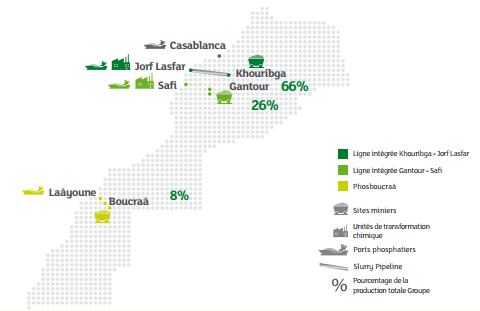
\includegraphics[width=0.9\textwidth]{./images/sites_ocp.png}
    \caption{Site de production}
\end{figure}

\paragraph{\textcolor{ocp}{Sites d'extraction phosphatière :}}
\begin{itemize}[label=$\bullet$]
    \item Boucraâ-Laâyoune, Khouribga, Youssoufia, Benguerir.
\end{itemize}

\paragraph{\textcolor{ocp}{Sites de transformation chimique :}}
\begin{itemize}[label=$\bullet$]
    \item Safi, Jorf Lasfar.
\end{itemize}
% chaine_ocp.png
\begin{figure}[H]
    \centering
    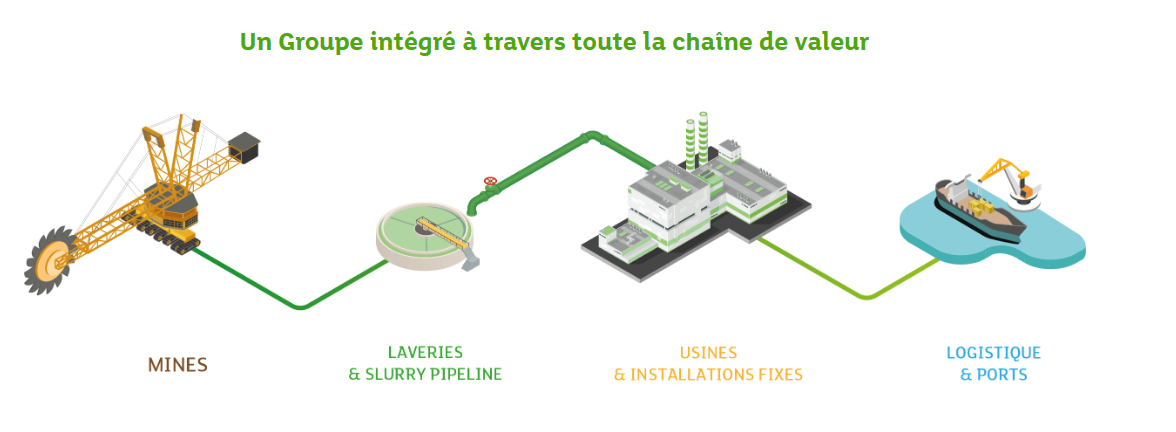
\includegraphics[width=0.9\textwidth]{./images/chaine_ocp.png}
    \caption{Chaine de production}
\end{figure}

\section{PHOSBOUCRAA }
Cette entreprise représente une société anonyme au sein du Groupe \texttt{OCP}, dont l'activité opérationnelle est menée par une équipe multidisciplinaire composée d'ingénieurs et assimilés, de techniciens de maîtrise, d'ouvriers spécialisés et d'employés administratifs.

\subsection{Organisation en divisions spécialisées}
\textsc{Phosboucraa} structure ses activités autour de trois divisions complémentaires :

\subsubsection{Division Extraction et Exploitation}
\begin{notebox}
\textbf{Localisation :} Située à 100 km au Sud-est de Laâyoune, précisément à Boucraâ
\end{notebox}

Cette division assure l'extraction et l'exploitation des phosphates en utilisant un matériel hautement performant et adapté aux conditions d'exploitation spécifiques du site. Elle comprend :
\begin{itemize}[label=$\bullet$]
    \item La mine à ciel ouvert
    \item Le parc matériel et équipements
    \item Les ateliers de maintenance
    \item Le campement résidentiel du personnel
\end{itemize}

Le transport du phosphate vers la plage s'effectue via un système de bandes transporteuses de 110 km, appelé « convoyeur », divisé en dix sections télécommandées par un système de télétransmission sophistiqué.

\begin{figure}[H]
    \centering
    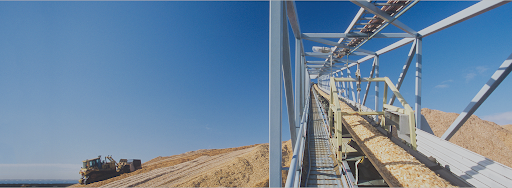
\includegraphics[width=0.9\textwidth]{./images/conveyor_ocp.png}
    \caption{Convoyeur}
\end{figure}

\subsubsection{Division Traitement}
\begin{notebox}
\textbf{Localisation :} Environ 32 km au Sud-ouest de Laâyoune
\end{notebox}

Cette division a pour mission de :
\begin{itemize}[label=$\bullet$]
    \item Réceptionner le phosphate brut en provenance de Boucraâ
    \item Traiter et enrichir le minerai
    \item Préparer l'exportation via les moyens de transport maritime
\end{itemize}

\subsubsection{Division Administrative}
Basée à Laâyoune, cette division centralise l'ensemble des services support :

\begin{table}[H]
\centering
\begin{tabular}{|l|p{8cm}|}
\hline
\textbf{\color{ocp}Service} & \textbf{Missions principales} \\
\hline
\texttt{Gestion Administrative} & Coordination administrative générale \\
\hline
\texttt{Service Médical} & Suivi sanitaire du personnel \\
\hline
\texttt{Analyses et Finances} & Gestion financière et analytique \\
\hline
\texttt{Service Social} & Accompagnement social des employés \\
\hline
\texttt{Approvisionnement} & Gestion des achats et stocks \\
\hline
\texttt{Formation et Devloppement RH} & Développement des compétences \\
\hline
\texttt{Service Informatique} & Technique et développement \\
\hline
\texttt{Service Juridique} & Assistance juridique et contentieux \\
\hline
\end{tabular}
\caption{Services de la Division Administrative}
\end{table}

\subsection{Contexte et problématique}
\hspace{.8cm} Gestion manuelle des stages : emails, tableurs, absence de suivi centralisé.

\subsection{Objectifs du projet}
\hspace{.8cm} Présentation des objectifs majeurs du projet.

\subsection{Méthodologie de travail adoptée}
\hspace{.8cm} Ex. Agile/Scrum, sprints, démarche adoptée.

\subsection{Planification prévisionnelle}
\hspace{.8cm} Diagramme de Gantt et calendrier du projet.

\newpage
% ─────────────────────────────────────────────────────────
\section{Étude et analyse des besoins}

\subsection{Étude de l'existant et critique}
\hspace{.8cm} Analyse des processus actuels et limitations identifiées.

\subsection{Identification des acteurs}
\hspace{.8cm} Étudiant/Candidat, Encadrant, Administrateur — rôles et responsabilités.

\subsection{Besoins fonctionnels par acteur}
\hspace{.8cm} Détail des fonctionnalités attendues pour chaque type d'utilisateur.

\subsection{Besoins non fonctionnels}
\hspace{.8cm} Sécurité JWT, ergonomie, performance, disponibilité.

\subsection{Diagramme de cas d'utilisation}
\hspace{.8cm} Représentation graphique des interactions entre acteurs et système.

\newpage
% ─────────────────────────────────────────────────────────
\section{Conception}

\subsection{Architecture générale}
\hspace{.8cm} Architecture 3-tiers : Angular / Spring Boot / MySQL.

\subsection{Justification des choix technologiques}
\hspace{.8cm} Analyse des alternatives et justification des technologies sélectionnées.

\subsection{Modèle conceptuel de données}
\hspace{.8cm} MCD/MLD et structure de la base de données.

\subsection{Diagramme de classes}
\hspace{.8cm} Représentation du modèle objet et des relations entre entités.

\subsection{Diagrammes de séquence}
\hspace{.8cm} Séquences d'interaction pour les fonctionnalités clés.

\subsection{Diagramme de déploiement}
\hspace{.8cm} Architecture d'infrastructure et déploiement de l'application.

\newpage
% ─────────────────────────────────────────────────────────
\section{Réalisation}

\subsection{Environnement de travail}
\hspace{.8cm} IDE, outils, versions : Java 21, Angular 21, MySQL.

\subsection{Technologies utilisées}
\hspace{.8cm} Spring Security/JWT, Spring Data JPA, OpenPDF, RxJS, et autres librairies clés.

\subsection{Architecture du backend}
\hspace{.8cm} Couches controller/service/repository/entity, DTOs.

\subsection{Architecture du frontend}
\hspace{.8cm} Composants standalone, routing, guards, polling temps réel.

\subsection{Captures d'écran commentées}
\hspace{.8cm} Présentation de l'interface par rôle et fonctionnalité.

\subsection{Zoom sur les fonctionnalités notables}
\subsubsection{Candidature sans compte}
\hspace{.8cm} Processus d'application sans authentification préalable.

\subsubsection{Verrouillage d'évaluation}
\hspace{.8cm} Mécanisme de confirmation et verrouillage des évaluations.

\subsubsection{Génération PDF de l'attestation}
\hspace{.8cm} Création automatique des documents finaux.

\subsubsection{Upload de CV}
\hspace{.8cm} Gestion des fichiers et stockage des pièces jointes.

\newpage
% ─────────────────────────────────────────────────────────
\section{Tests et validation}

\subsection{Stratégie et types de tests}
\hspace{.8cm} Plan de test global : unitaires, intégration, fonctionnels, utilisateur.

\subsection{Scénarios de test par rôle}
\hspace{.8cm} Détail des cas de test pour chaque profil d'utilisateur.

\subsection{Difficultés rencontrées et solutions apportées}
\hspace{.8cm} Problèmes identifiés et approches de résolution employées.

\newpage
% ─────────────────────────────────────────────────────────
\section*{Conclusion générale et perspectives}

\hspace{.8cm} Bilan du projet, limites actuelles et améliorations futures.

\subsection*{Bilan}
\hspace{.8cm} Synthèse des objectifs atteints et des livrables produits.

\subsection*{Limites actuelles}
\hspace{.8cm} Points à améliorer et fonctionnalités non implémentées.

\subsection*{Améliorations futures}
\hspace{.8cm} Notifications par email, tests automatisés, optimisations proposées.

\newpage
% ─────────────────────────────────────────────────────────
\section*{Bibliographie / Webographie}

\hspace{.8cm} Ressources, références documentaires et sources consultées.

\newpage
% ─────────────────────────────────────────────────────────
\section*{Annexes}

\hspace{.8cm} Documents supplémentaires, schémas détaillés, extraits de code, données brutes.

\end{document}